\section{Messung}\label{kap:measurements}

Der Tisch ist an den Seiten leicht schräg, was ein genaues Messergebnis verunmöglicht. Weiterhin ist er an den Kanten
nicht fest und kann leicht deformiert werden. Um diese Ungenauigkeitsfaktoren möglichst gering zu halten, wurden die
gegenüberliegenden Tischkanten mit je zwei Holzstücken (Abbildung \ref{fig:messung:tisch}, 1), deren Breite individuell
über einen Messschieber millimetergenau bestimmt wurde, ausgestattet. Nun kann die Distanz zwischen den Holzstücken
gemessen und anschliessend die Breite der Hölzer dazuaddiert werden. Die Messung selbst (Abbildung \ref{fig:messung:tisch}, 2 und 3)
wird über ein Laser-Messgerät\footnote{Die genauen Spezifikationen sind im Anhang \ref{anhang:messung:messgeraete} ersichtlich.}
durchgeführt. Die Messungenauigkeit wird mit $\pm 1.5mm$ angegeben. Die Abbildung \ref{fig:messung:tisch} zeigt die Messung in X-Richtung,
diese Messung wird ebenfalls in gleicher Art und Weise in Y-Richtung durchgeführt.
\begin{figure}[h!]
    \begin{center}
        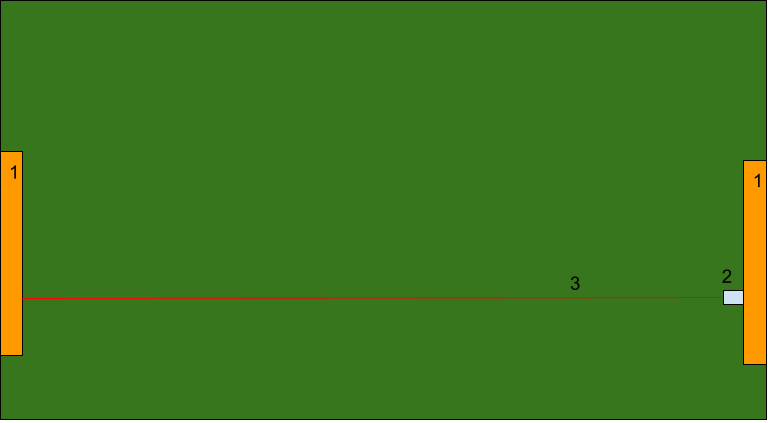
\includegraphics[width=0.6\linewidth]{../common/03_billiard_ai/resources/01_messung_tisch.png}
    \end{center}
    \caption{Messung - Tisch}
    \label{fig:messung:tisch}
\end{figure}


Um die Messung der Kugeln zu erläutern, muss zuerst das Koordinatensystem eingeführt werden. Die Kugeln selbst werden
über eine Kamera aufgenommen und deren Position daher auch in einem Pixelkoordinatensystem bestimmt. Dies ist aus
mehreren Gründen ungünstig. Einerseits soll die allgemeine Abhängigkeit zur Kamera vermieden werden, andererseits ist das
Pixelkoordinatensystem für die Visualisierung nicht gut geeignet.\\
Die Kugeln werden also in ein Modellkoordinatensystem übersetzt\footnote{Siehe Kapitel \ref{kap:model_coordinate_system}}.
Bei diesem befindet sich der Ursprung in der Mitte des Tisches und die X- wie auch die Y-Achse bilden die Breite und Höhe
in Millimeter ab.

Um nun die Position der Kugel zu bestimmen, wird zuerst deren Abstand zu den Banden gemessen (siehe Abbildung \label{fig:messung:kugel}, 1 und 2).
Dies geschieht wie beim Ausmessen des Tisches über ein Holzstück und das Lasermessgerät. Wurden beide Distanzen bestimmt, so
kann der Mittelpunkt der Kugel berechnet werden, indem noch der Radius, welcher durch einen Messschieber bestimmt wurde, dazuaddiert wird.
Es gilt nun, diesen Punkt in das Modellkoordinatensystem zu übersetzen. Dazu wird jeweils die halbe Breite wie auch Höhe
(beachte den Ursprung des Modellkoordinatensystems) von dem Mittelpunkt abgezogen. Abschliessend werden noch die korrekten
Vorzeichen über den Quadranten bestimmt.

\begin{figure}[h!]
    \begin{center}
        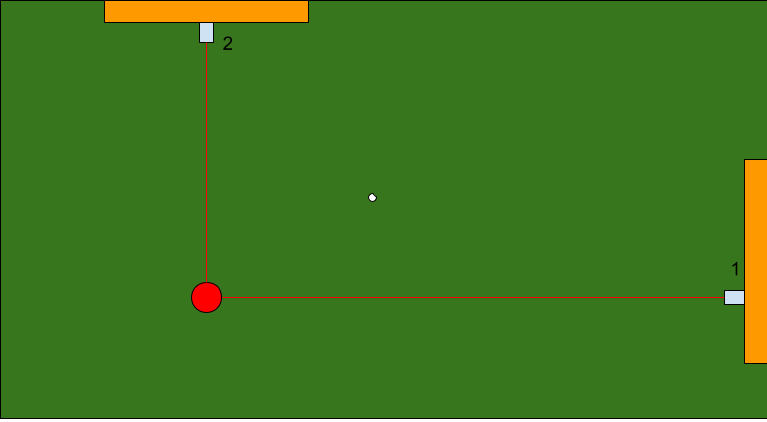
\includegraphics[width=0.6\linewidth]{../common/03_billiard_ai/resources/02_messung_kugel.png}
    \end{center}
    \caption{Messung - Kugel}
    \label{fig:messung:kugel}
\end{figure}
